\documentclass[a4paper,10pt]{article}

\usepackage[utf8x]{inputenc}
\usepackage{amsfonts}
\usepackage{amsmath}
\usepackage[french]{babel}
\usepackage{xspace}
\usepackage{lmodern}
\usepackage[babel]{microtype}
\usepackage[T1]{fontenc}
\usepackage{graphicx}
\usepackage{epsfig}
\usepackage{fullpage}

\author{David Hauweele}
\title{Synthèse Analyse}
\date{2007-10-23}

%%\newcommand{\mod}{\mbox{ mod }}

\newcommand{\rd}{\circ}
%%\newcommand{\sin}{\mbox{sin }}
%%\newcommand{\cos}{\mbox{cos }}
%%\newcommand{\tan}{\mbox{tan }}
%%\newcommand{\arcsin}{\mbox{arcsin }}
%%\newcommand{\arctan}{\mbox{arctan }}
\newcommand{\Adh}{\mbox{ Adh }}
\newcommand{\Bd}{\mbox{ Bd }}
\newcommand{\Int}{\mbox{ Int }}
\newcommand{\Maj}{\mbox{ Maj }}
\newcommand{\ap}{\rightarrow}
\newcommand{\nap}{ \longrightarrow {\kern-13,5pt{\backslash}}~~}
\newcommand{\apw}[1]{\stackrel{#1}{\rightarrow}}
\newcommand{\Dom}{\mathrm{Dom}\:}
\newcommand{\R}{\mathbb{R}}
\newcommand{\C}{\mathbb{C}}
\newcommand{\N}{\mathbb{N}}
\newcommand{\Q}{\mathbb{Q}}
\newcommand{\Z}{\mathbb{Z}}
\newcommand{\so}{\Rightarrow}
\newcommand{\os}{\Leftarrow}
\newcommand{\ioi}{\Leftrightarrow}
\newcommand{\tset}[1]{\left\lbrace #1 \right\rbrace}
\newcommand{\conv}[1]{\mathop{\longrightarrow}\limits_{#1}}
\newcommand{\nconv}[1]{\mathop{\nap}\limits_{#1}}
\newcommand{\abs}[1]{\left\vert #1 \right\vert}
\newcommand{\ceil}[1]{\left\lceil #1 \right\rceil}
\newcommand{\norme}[1]{\parallel #1 \parallel}
\newcommand{\clim}[1]{\lim\limits_{#1}}
\newcommand{\but}{\setminus}
\newcommand{\Id}{\mbox{Id}}
\newcommand{\cclass}[3]{\mathcal{C}^{#1} (#2;#3)}
\newcommand{\Poly}{\mathbb{P}}
\newcommand{\series}{\sum_{n=n_0}^{+\infty}}
\newcommand{\Series}[1]{\sum_{n=#1}^{+\infty}}
\newcommand{\eqdo}{EDO }

\begin{document}

\maketitle
Last revision : \today

%Document réalisé en \LaTeX

%Document réalisé sous Vim

%Figures réalisées sous XFig

%Le tout sur Linux et FreeBSD
\tableofcontents
\newpage
\section{Limites et continuité}

\subsection{Suite}
Une suite est une fonction\footnote{C'est une fonction dite discrete car $I \subseteq \N$.} $I \rightarrow \mathbb{R} : n \mapsto x_n$ où $I = \left\lbrace n \in \mathbb{N} : n \geq n^* \right\rbrace$ pour un certain $n^*$ dépendant de $I$.

On note\footnote{C'est un abus de notation, on sous entend en fait que l'ensemble des éléments de la suite est inclu ou égal à $\mathbb{R}$.} $(x_n)_{n \in I} \subseteq \mathbb{R}$ pour parler de la suite $I \rightarrow \R : n \mapsto x_n$.

\subsection{Suite arithmétique}

Une suite $(x_n)_{n\in \N^{~>k}}$ est arithmétique s'il existe deux réels $a$ et $r$ tel que :

$\begin{cases} x_k = a\\ x_n = x_{n-1} +r\end{cases}$

Avec $r$ appelé la raison de la suite.

Une définition équivalente est 

$$\exists a,r \in \R : x_n = a + (n-k)r $$

\subsection{Suite géométrique}

Une suite $(x_n)_{n\in I}$ est géométrique s'il existe deux réels $a$ et $r$ tel que : 

$\begin{cases} x_k = a\\ x_n=x_{n-1} r\end{cases}$

Avec $r$ est appelé la raison de la suite.

Une définition équivalente est

$$\exists a,r \in \R : x_n = a r^{n-k}$$

\subsection{Notion de convergence}

Une suite $(x_n)_{n \in I}$ est dite \textit{converger} ou \textit{tendre} vers $l \in \mathbb{R}$,ce qu'on note $x_n \conv{n \ap \infty} l$, ssi :

$$\forall \varepsilon > 0, \exists n_0 \in I, \forall n \geq n_0, x_n \in \left[ l - \varepsilon , l + \varepsilon \right]$$
$$\Updownarrow$$
$$\forall \varepsilon > 0, \exists n_0 \in I, \forall n \geq n_0, x_n \in \vert x_n - l \vert \leq \varepsilon$$

Ex:

$$\frac{1}{n} \conv{n \ap \infty} 0$$
$$\mbox{? } \forall \varepsilon > 0, \exists n_0, \forall n \geq n_0, \left\vert \frac{1}{n} \right\vert < \varepsilon$$

\underline{Preuve} : 

Soit $\varepsilon > 0$ arbitraire, indép. de $n_0,n$

Prenons $n_0 = \ceil{\frac{1}{\varepsilon}} \in \N$

Soit $n \geq n_0$ arbitraire

On a $n \geq \ceil{\frac{1}{\varepsilon}} \geq \frac{1}{\varepsilon}$

Donc $n \geq \frac{1}{\varepsilon}$ i.e. $\frac{1}{n} \leq \varepsilon$

Comme $\frac{1}{n} > 0$, on conclu que $\left\vert \frac{1}{n} \right\vert \leq \varepsilon$ 

%\newpage

Ex :

$$\frac{1}{n} \nconv{n \ap \infty} 1$$

$$\mbox{? } \exists \varepsilon > 0, \forall n_0, \exists n \geq n_0, \abs{\frac{1}{n} -1} > \varepsilon$$

\underline{Preuve} :

Prenons $\varepsilon = \frac{1}{2}$

Soit $n_0$ arbitraire

Prenons $n = \max\tset{3, n_0}$

Donc $n \geq 3$ d'où $\frac{1}{n} \leq \frac{1}{3}$ d'où $1 - \frac{1}{n} \geq 1 - \frac{1}{3} = \frac{2}{3}$

e.p. $1 - \frac{1}{n} \geq 0, \abs{1-\frac{1}{n}} = 1 - \frac{1}{n} \geq \frac{2}{3} > \frac{1}{2}$

\subsection{Notation limite}
Soit $(x_n)_{n \in I}$, on appelle $\lim\limits_{n \ap \infty} x_n$ le nombre\footnote{Le symbole $\lim$ requiert l'unicité des limites. Voir démonstration au cours.} $l$,\textit{s'il existe}, tel que $x_n \conv{n \ap \infty} l$.

\subsection{Opération sur les suites}

\subsubsection{Somme}
$$(x_n + y_n)_{n \in I \cup J} =: (x_n)_{n \in I} + (y_n)_{n \in J}$$

Autrement dit :

$$(x_n) : I \ap \R : n \mapsto x_n$$
$$(y_n) : J \ap \R : n \mapsto y_n$$
$$(x_n + y_n) : I \cap J \ap \R : n \mapsto x_n + y_n$$ 


\subsubsection{Produit}
$$(x_n . y_n)_{n \in I \cap J} =: (x_n)_{n \in I} . (y_n)_{n \in J}$$

Autrement dit :

$$(x_n) : I \ap \R : n \mapsto x_n$$
$$(y_n) : J \ap \R : n \mapsto y_n$$
$$(x_n . y_n) : I \cap J \ap \R : n \mapsto x_n . y_n$$

\subsubsection{Remarque}

Des opérations sur les suites on retire que l'ensemble des suites sur $\R$ càd $S = \tset{x \vert x = (x_n)_{n \in I} \subseteq \R}$ forme un espace vectoriel de dimension infinie.

En effet l'opération $+$ est définie et $\alpha(x_n)_{n \in I} := (\alpha x_n)_{n \in I}$.

Notons aussi que $S \apw{\lim} \R : (x_n) \mapsto \lim\limits_{n\ap\infty} x_n$ est une application $\R$-linéaire.

\subsection{Opération arithmétiques sur les limites}
Soit $(x_n)_{n\in I} \subseteq \R$ et $(y_n)_{n \in J} \subseteq \R$ et $l,l' \in \R$

Si $x_n \ap l$ et $y_n \ap l'$ 
\subsubsection{Somme}
Alors $x_n \pm y_n \ap l \pm l'$

Càd $\lim\limits_{n\ap\infty} x_n + y_n = \lim\limits_{n\ap\infty} x_n + \lim\limits_{n\ap\infty} y_n$
\subsubsection{Produit}
Alors $x_n . y_n \ap l . l'$

Càd $\lim\limits_{n\ap\infty} x_n . y_n = \lim\limits_{n\ap\infty} x_n . \lim\limits_{n\ap\infty} y_n$
\subsubsection{Quotient}
Si $l' \neq 0$ alors $\frac{x_n}{y_n} \ap \frac{l}{l'}$

Càd $\lim\limits_{n\ap\infty} \frac{x_n}{y_n} = \frac{\lim\limits_{n\ap\infty} x_n}{\lim\limits_{n\ap\infty} y_n}$

\subsubsection{Remarque}

Quand on dit par exemple $\lim\limits_{n\ap\infty} x_n + y_n = \lim\limits_{n\ap\infty} x_n + \lim\limits_{n\ap\infty} y_n$ on suppose les limites $\lim\limits_{n\ap\infty} x_n$ et $\lim\limits_{n\ap\infty} y_n$ existent.

\subsubsection{Convergence dominée}

Soit $(x_n)_{n \in I}$ et $l \in \R$ si $\exists n^\star, \forall n \geq n^\star, \abs{x_n - l} \leq y_n$ et $y_n \ap 0$ on a $x_n \ap l$

Ex : 

$$\abs{\frac{(-1)^n}{n}} = \frac{1}{n} \ap 0$$

Ex :

$$x_n = \frac{n+(-1)^n}{n+\sqrt{n}} \so \abs{x_n -1} = \abs{\frac{n+(-1)^n-n-\sqrt{n}}{n+\sqrt{n}}} \leq \frac{\abs{(-1)^n}+\abs{\sqrt{n}}}{n+\sqrt{n}} = \frac{1+\sqrt{n}}{n+\sqrt{n}} \leq 2\sqrt{n} = \frac{2}{\sqrt{n}} \conv{n \ap \infty} 0$$

\subsubsection{Théorème du Sandwich}

Soit $(x_n), (y_n), (z_n)$ trois suites et $l \in \R$ tq $\forall n y_n \leq x_n \leq z_n$

Si $y_n \ap l$ et $z_n \ap l$ alors $x_n \ap l$

\subsubsection{Suites de bases pour les opérations sur les limites}

\begin{itemize}
	\item{$\frac{1}{n^\alpha} \ap 0$ si $\alpha > 0$}
\end{itemize}


\subsubsection{Suite bornée}

Une suite $x_n$ est bornée ssi $\exists C \geq 0, \forall n \in I, \abs{x_n} \leq C$

Ex: $\frac{1}{n}$ est bornée car on a $\forall n \in I, \abs{\frac{1}{n}} \leq 1$

\subsubsection{Proposition}

Si une suite converge alors elle est bornée

Si $(x_n)$ n'est pas bornée et $y_n \ap l \neq 0$ alors $\left( \frac{x_n}{y_n} \right)$ n'est pas bornée

\subsubsection{Limites d'inégalités}

Si $(x_n)$ et $(y_n)$ tq $x_n \ap l \in \R$ et $y_n \ap l' \in \R$ et $\exists n^\star, \forall n \geq n^\star, x_n \leq y_n$ alors $l \leq l'$

\paragraph{Remarque} Par passage à la limite, les inégalités strictes deviennent larges.

\subsection{Divergence}

\subsubsection{Sous-suite}

Une suite $(y_n)_{n\in J}$ est dite sous-suite de $(x_n)_{n \in I}$ ssi il existe une fonction $\varphi : J \ap I$ tq $\forall k \in J, y_k = x_{\varphi(k)}$ et $\varphi$ est strictement croissante, càd $\forall k, \varphi(k) < \varphi(k+1)$

On note\footnote{C'est un abus de notation voir la notation $(x_n) \subseteq \R$.} $(y_n) \subseteq (x_n)$ pour dire que $(y_n)$ est une sous-suite de $(x_n)$

\subsubsection{Strictement croissant}

Une fonction $f : A \ap B$ est strictement croissante ssi $$\forall a,a' \in A, a < a' \so f(a) < f(a')$$

$$\Downarrow$$

Pour les fonctions $\N \ap \R$ comme les suites on peut dire $$\forall k \in \N, x_k < x_{k+1}$$

\subsubsection{Convergence des sous-suites}

Si $(y_n) \subseteq (x_n)$ et $x_n \ap l$ alors $y_n \ap l$

\subsubsection{Proposition}

Si $(x_n) \subseteq \R^{>0}, x_n \ap 0$ alors $\exists (y_n) \subseteq (x_n) : (y_n) \searrow \searrow$

Si $(x_n) \subseteq \R, x_n \ap l$ alors $\exists (y_n) \subseteq (x_n) : (y_n)$ est monotone


\subsection{Convergence au sens large}

La suite $(x_n) \subseteq \R$ converge vers $+\infty$ ssi $\forall \varphi > 0, \exists n_0, \forall n \geq n_0, x_n \geq \varphi$

On note $x_n \ap +\infty$

La suite $(x_n) \subseteq \R$ converge vers $-\infty$ ssi $\forall \varphi < 0, \exists n_0, \forall n \geq n_0, x_n \leq \varphi$

On note $x_n \ap -\infty$

Remarque :

On a $x_n \ap -\infty \ioi -x_n \ap +\infty$

\subsubsection{Convergence dominée au sens large}

Si $(x_n)$ et $(y_n$ deux suites tq $\forall x_n \geq y_n$ et $y_n \ap +\infty$, alors $x_n \ap +\infty$

\subsubsection{Opération sur les limites au sens large}

\begin{itemize}
	\item{$x_n \ap \pm \infty, y_n \ap \pm \infty \so x_n + y_n \ap \pm \infty$}
	\item{$x_n \ap \pm \infty, y_n \ap \mp \infty \so x_n + y_n \ap +\infty \mbox{ ou } x_n + y_n \ap -\infty \mbox{ ou } x_n + y_n \ap l \mbox{ ou } x_n + y_n \mbox{ diverge}$}
	\item{$x_n \ap \pm \infty, y_n \ap \pm \infty \so x_n . y_n \ap +\infty$}
	\item{$x_n \ap \pm \infty, y_n \ap \mp \infty \so x_n . y_n \ap -\infty$}
	\item{$x_n \ap +\infty, y_n \ap l > 0 \so x_n . y_n \ap +\infty$}
	\item{$x_n \ap -\infty, y_n \ap l < 0 \so x_n . y_n \ap +\infty$}
	\item{$x_n \ap +\infty, y_n \ap l < 0 \so x_n . y_n \ap -\infty$}
	\item{$x_n \ap -\infty, y_n \ap l > 0 \so x_n . y_n \ap -\infty$}
	\item{$x_n \ap \pm \infty, y_n \ap l = 0 \so x_n . y_n \ap +\infty \mbox{ ou } x_n . y_n \ap -\infty \mbox{ ou } x_n . y_n \ap l' \mbox{ ou } x_n . y_n \mbox{ diverge}$}
	\item{$x_n \ap \pm \infty \so \frac{1}{x_n} \ap 0$}
	\item{$x_n \ap 0, (x_n) \subseteq \R^{<0} \so \frac{1}{x_n} \ap -\infty$}
	\item{$x_n \ap 0, (x_n) \subseteq \R^{>0} \so \frac{1}{x_n} \ap +\infty$}
\end{itemize}

\subsubsection{Bornée inférieurement}

La suite $(x_n)$ est bornée inférieurement en $C$ ssi $\forall n, x_n \geq C$

\subsubsection{Bornée supérieurement}

La suite $(x_n)$ est bornée supérieurement en $C$ ssi $\forall n, x_n \leq C$

\subsection{Minimum}
$\min A = a \ioi a \in A, \forall x \in A, a \leq x$

Note : $\min \R$ n'existe pas alors que $\min \R \cup \tset{+\infty, -\infty} = -\infty$

\subsection{Maximum}

$\max A = a \ioi a \in A, \forall x \in A, a \geq x$

Note : $\max \R$ n'existe pas alors que $\max \R \cup \tset{+\infty, -\infty} = +\infty$

\subsubsection{Proposition}

Si $A$ est fini alors $\min A$ existe.

Si $A$ est fini alors $\max A$ existe.

$\max \emptyset = +\infty$

$\min(A) = -\max(-A)$

\subsection{Ordre étendu}

$$\forall x \in \R, -\infty < x < +\infty$$

\subsection{Réels étendus}

On note $\bar \R = \R \cup \tset{+\infty, -\infty} = \left[ -\infty, +\infty \right]$

Note : On a $\R \subseteq \bar \R$

Note : Si $x,y \in \R, x \leq_\R y \ioi x \leq_{\bar \R} y$

\subsection{Méthode de Newton}

Soit une fonction $f(x)$, on cherche la racine.

Soit $(x_n)$ définie par récurrence tq $x_0 \in \mbox{Dom } f$ et $x_{n+1} = x_n - \frac{f(x_n)}{\partial f(x_n)}$

Alors $f\left( \lim\limits_{n \ap \infty} x_n \right)$ est racine. 

\subsection{Suite de Cauchy}

Une suite $(x_n)$ est de Cauchy ssi $\forall \varepsilon > 0, \exists n_0, \forall n,m \geq n_0, \vert x_n - x_m \vert \leq \varepsilon$

\subsection{Proposition}

Si $(x_n)$ et $(y_n)$ sont de Cauchy alors $(x_n + y_n)$ est de Cauchy

Si $(x_n)$ et $(y_n)$ sont de Cauchy alors $(x_n.y_n)$ est de Cauchy

Si $(x_n)$ et $(y_n)$ sont de Cauchy alors $\left( \frac{x_n}{y_n} \right)$ est de Cauchy

$(x_n)$ est de Cauchy $\ioi (x_n)$ est strictement convergente

\subsubsection{Critère de convergence}

Si $(x_n)$ est une suite, $(x_n)$ est bornée inf. et $(x_n) \downarrow \so (x_n)$ est de Cauchy $\so (x_n)$ est strictement convergente

Si $(x_n)$ est une suite, $(x_n)$ est bornée sup. et $(x_n) \uparrow \so (x_n)$ est de Cauchy $\so (x_n)$ est strictement convergente

\subsubsection{Critère d'équivalence}

Une suite $(x_n)_{n\in I}$ est équivalente à $(y_n)_{n\in J}$ si $\lim\limits_{n\ap \infty} \frac{x_n}{y_n} = 1$ ce qu'on note $(x_n) \sim (y_n)$

\subsubsection{Proposition}

Si $y_n \ap a$ et $x_n \sim y_n$ alors $x_n \ap a$
\subsubsection{Notion de réel}

$$\R = \frac{\tset{\mbox{ensemble des suites de Cauchy}}}{(x_n) \sim (y_n)}$$

où $\sim =$ avoir même limite

\subsubsection{Définition de réel}

$\R$ est le plus petit ensemble contenant $\Q$ et toutes les limites de suite de cauchy de $\Q$ (et donc dans $\R$)

\subsubsection{Espace complet} 

Un espace $X$ est complet ssi toute suite de Cauchy $(x_n) \subseteq X$ possède une limite dans $X$

Eg : $\R$ est le plus petit espace complet contenant $\Q$

\subsubsection{Définition concrète de réel}

$\R = \tset{ d_N d_{N-1} \cdots d_1 d_0, d_{-1} d_{-2} \cdots}$ où on identifie un nombre qui se termine par une suite de 9 à un nombre qui se termine par une suite de 0 selon la règle précédente (eg. $0,99\cdots = 1$)

\subsubsection{Densité}

On dit que $X$ est dense dans $Y$ ssi $\forall y \in Y, \exists (x_n) \subseteq X$ tq $x_n \ap y$

Eg: 

$\Q$ est dense dans $\R$

$\R$ est dense dans $\bar \R$

$\left] 0, 1 \right[$ est dense dans $\left[ 0,1\right]$
(on ajoute le bord)

\subsection{Supremum}

$a$ est suprémum de $A$ ssi:

$\forall \varepsilon > 0, \left[ a - \varepsilon,a \right] \cap A \neq \emptyset$

$\forall x \in A, x \leq a$

Noté $\sup A = a$

\subsubsection{Définition équivalente}

$\sup A = a$ ssi:

$\forall \varepsilon > 0, \exists a' \in A, a' \geq a - \varepsilon$

$\forall x \in A, x \leq a$

\subsubsection{Définition équivalente}

$\sup A = a$ ssi:

$\exists (a_n) \subseteq A, a_n \ap a$

$\forall x \in A, x \leq a$

\subsection{Infimum}

$a$ est infimum de $A$ ssi:

$\forall \varepsilon > 0, \left[ a + \varepsilon,a \right] \cap A \neq \emptyset$

$\forall x \in A, x \geq a$

Noté $\inf A = a$

\subsubsection{Définition équivalente}

$\inf A = a$ ssi:

$\forall \varepsilon > 0, \exists a' \in A, a' \leq a + \varepsilon$

$\forall x \in A, x \geq a$

\subsubsection{Définition équivalente}

$\inf A = a$ ssi:

$\exists(a_n) \subseteq A, a_n \ap a$

$\forall x \in A, x \geq a$

\subsection{Proposition}

Si $\max A$ existe alors $\sup A = \max A$

Si $\min A$ existe alors $\inf A = \min A$

$\inf(A) = -\sup(-A)$

$\sup A = \min \Maj(A)$

Si $A \neq \emptyset$ et est borné supérieurement alors $\sup A$ existe

%%\subsubsection{Lemme}

%%$a$ est supremum de $A$ ssi

%%$\exists(a_n) \subseteq A, a_n \ap a$

%%$\forall x \in A, x \leq a$

\subsubsection{Lemme}

Soit $A \neq \emptyset$ est borné supérieurement et $\delta > 0$, alors $\exists a \in A, a + \delta$ majore $A$

\subsubsection{Majorant}

$x\in \R$ est majorant de $A \subseteq \R$ ssi $\forall a \in A, x \geq a$

On note $\Maj(A)$ l'ensemble des majorants de $A$

\subsubsection{Minorant}

$x\in \R$ est minorant de $A \subseteq \R$ ssi $\forall a \in A, x \leq a$

\subsection{Suites de base}


\subsubsection{Suite du type $a^n$}
\begin{itemize}
	\item[$\abs{a} < 1$]{Converge vers 0}
	\item[$a=1$]{Converge vers 1}
	\item[$a>1$]{Converge au sens large vers $+\infty$}
	\item[$a \leq -1$]{Ne converge pas}
\end{itemize}

\subsubsection{Suite du type $n^k.a^n$}

\begin{itemize}
	\item[$\abs{a} < 1$]{Converge vers 0}
\end{itemize}


\subsubsection{Suite du type $\frac{a^n}{n!}$}

$\forall a, \frac{a^n}{n!} \ap 0$

\subsection{Généralisation à $\R^{N}$}

\subsubsection{Notion de suite}

Une suite de vecteur de $\R^N$ est une fonction $x : I \ap \R^N$ où $I = \tset{n \in \N : n \geq n_I}$ pour un $n_I \in \N$

On note\footnote{Attention à l'abus de notation, voir la remarque pour les suites dans $\R$.} $x_n$ pour $x(n) \in \R^N$ et $(x_n)_{n\in I} \subseteq \R^N$ au lieu de $x : I \ap \R^N$


\subsubsection{Notion de norme}

Une norme sur $\R^N$ est une fonction $\norme{.} : \R^N \ap \R^{\geq 0}$ qui vérifie les propriétés suivantes :

\begin{enumerate}
\item{$\forall x \in \R^N, \norme{x} = 0 \so x = 0$}
\item{$\forall x \in \R^N, \forall \lambda \in \R, \norme{\lambda x} = \abs{\lambda}.\norme{x}$}
\item{$\forall x,y \in \R^N, \norme{x+y} \leq \norme{x} + \norme{y}$}
\end{enumerate}

\subsubsection{Propriétés sur la norme}

\begin{itemize}
	\item{$\exists \alpha \in \R^{>0}, \forall x \in \R, \norme{x} = \alpha \abs{x}$}
	\item{$\norme{0} = 0$}
	\item{$\abs{\norme{x} - \norme{y}} \leq \norme{x - y}$}
\end{itemize}

\subsubsection{Norme Euclidienne}

On note $\abs{.}_2$ la norme Euclidienne tq $\forall x \in \R^N, \abs{x}_2 = \sqrt{\sum_{i=1}^N x_i^2}$

Remarque : $\abs{x}_2 = \sqrt{(x \vert x)}$ avec $(x \vert y) = \sum_{i=1}^N x_i y_i$
\subsubsection{Taxi-distance}

On note $\abs{.}_1$ la norme Euclidienne tq $\forall x \in \R^N, \abs{x}_1 = \sum_{i=1}^N \abs{x_i}$

\subsubsection{Norme sup}

On note $\abs{.}_\infty$ la norme sup tq $\forall x \in \R^N, \abs{x}_\infty = \max \tset{\abs{x_1}, \cdots, \abs{x_N}}$

\subsubsection{Notion de convergence}

Une suite $(x_n)_{n\in I} \subseteq \R^N$ converge vers $a \in \R^N$ ssi

$$\forall \varepsilon > 0 , \exists n_0 \in \N, \forall n \geq n_0,\parallel x_n - a \parallel < \varepsilon$$

En dimension finie la convergence ne dépend pas de la norme

\subsubsection{Produit scalaire sur $\R^N$}

Un produit scalaire sur $\R^N$ est une fonction 

$$(. \vert .) : \R^N \times \R^N \ap \R : (x,y) \mapsto (x \vert y)$$

vérifiant :

\begin{enumerate}
	\item{La fonction est bilinéaire i.e. $\forall x \in \R^N, (x \vert .)$ linéaire et $\forall y \in \R^N,(. \vert y)$ linéaire}
	\item{La fonction est positive i.e. $\forall x \in \R^N, (x \vert x) \geq 0$}
	\item{La fonction est non dégénérée i.e. $\forall x \in \R^N, (x \vert x) = 0 \so x = 0$}
	\item{La fonction est symétrique i.e. $\forall x,y \in \R^N, (x \vert y) = (y \vert x)$}
\end{enumerate}

\subsection{Théorème de Cauchy-Schwarz}

$\abs{(x\vert y)} \leq \Vert x \Vert . \Vert y \Vert$ et $\Vert . \Vert : \R^N \ap \R^{\geq 0}$ est une norme

Quand on a $\abs{(x \vert y)} = \Vert x \Vert . \Vert y \Vert$ alors $x$ et $y$ sont linéairement dépendants (colinéaires).

\subsection{Matrice du produit scalaire dans la famille génératrice $(x,y)$}

On note la matrice du produit scalaire dans la famille génératrice $(x,y)$ de $\mbox{Vect} \tset{x,y}$ ou $\mbox{Span} \tset{x,y}$

$$
\begin{pmatrix}
(x \vert x) & (x \vert y) \\
(y \vert x) & (y \vert y)
\end{pmatrix}
$$

Le déterminant de cette matrice représente l'aire signée engendrée par les vecteurs $x$ et $y$

\subsection{Lemme}

$x_n \ap a \ioi \Vert x_n - a \Vert \ap 0$

\subsection{Opération sur les limites dans $\R^N$}

Soit $x_n \ap a$ et $y_n \ap b$ deux suites de $\R^N$
Soit $\lambda_n \ap l$ une suite de $\R$
On a :

$x_n + y_n \ap a + b$

$\lambda_n x_n \ap l.a$

$\frac{x_n}{\lambda_n} = \frac{1}{l} . x_n$
\subsection{Bornée dans $\R^N$}

La suite $(x_n) \subseteq \R^N$ est bornée ssi $\exists C \in \R, \forall n, \Vert x_n \Vert \leq C$

\subsection{Propriétés}

Si $(x_n) \subseteq \R^N$ converge alors $(x_n)$ est bornée

\subsection{Convergence dominée dans $\R^N$}

Soit $(x_n) \subseteq \R^N, a \in \R^N$ et $(y_n) \subseteq \R$ tq $\forall n, \Vert x_n - a \Vert \leq y_n$

Si $y_n \ap 0$ alors $x_n \ap a$

\subsection{Produits}

Un produit est $P : \R^N \times \R^M \ap \R^P$ tel que $P$ est bilinéaire

\subsubsection{Produits généraux}

\begin{itemize}
	\item[Multiplication par un scalaire]{$\R^N \times \R^N \ap \R : (\lambda, x) \mapsto \lambda.x$}
	\item[Produit scalaire]{$\R^N \times \R^N \ap \R : (x,y) \mapsto (x \vert y)$}
	\item[Produit vectoriel]{$\R^3 \times \R^3 \ap \R^3 : (x,y) \mapsto x \times y$}
	\item[Evaluation]{$\R^{N\times M} \times \R^M \ap \R^N : (A,x) \mapsto A.x$}
\end{itemize}

\subsubsection{Propriété}

Tous les produits sont continus (en dimension finie) càd 

$$\forall \left( \left( x_n,y_n \right) \right) \subseteq \R^N \times R^M \mbox{ et } \forall \left( a, b \right) \in \R^N \times \R^M$$

Si $x_n \ap a$ et $y_n \ap b$ alors $P(x_n,y_n) \ap P(a,b)$

\subsection{Norme dominée}

On dit que $\Vert. \Vert$ est dominée par $\Vert . \Vert'$ si

$\exists C > 0, \forall x, \Vert x \Vert \leq C \Vert x \Vert'$

\subsection{Normes équivalentes}

On dit que $\Vert . \Vert$ et $\Vert . \Vert'$ sont équivalentes si elles se dominent l'une l'autre

C'est une relation d'équivalence

\subsection{Théorème}

Si $\Vert.\Vert$ et $\Vert.\Vert'$ sont deux normes sur $\R^N$ avec $N < \infty$ alors $\exists C > 0, \forall x, \Vert x \Vert \leq C \Vert x \Vert'$ et donc aussi $\exists C' > 0, \forall x, \Vert x \Vert' \leq C' \Vert x \Vert$

\subsection{Norme sur $\R$}

Si $\Vert.\Vert$ est une norme sur $\R$ alors 

$\exists C > 0, \forall x \in \R, \Vert x \Vert = C \abs{x}$

\subsection{Propriété}

$$\forall x \in \R^N, \vert x \vert_\infty \leq \vert x \vert_2 \leq \vert x \vert_1 \leq N \vert x \vert_\infty$$

En fait, on a que, de façon optimale :

$$\forall x \in \R^N, \vert x \vert_\infty \leq \vert x \vert_2 \leq \vert x \vert_1 \leq N \vert x \vert_\infty$$

\subsubsection{$P_C$}

On a que $P_C$ est vérifié si $\forall x \in \R^N, \vert x \vert_2 \leq C.\vert x \vert_n$

\subsubsection{$C$ optimal}

On veut trouver le plus petit $C > 0$ tel que $P_C$

On prend le $C^* = \mbox{inf } \tset{C > 0 \vert (P_C)}$



\subsection{Boule ouverte}

On appelle boule ouverte de centre $a$ et de rayon $r$ pour la norme $\Vert . \Vert$ l'ensemble $B_{\Vert . \Vert} \left( a,r \right) = \tset{x \in \R^N \vert \mbox{  } \Vert x - a \Vert < r}$


\subsection{Boule fermée}

On appelle boule fermée de centre $a$ et de rayon $r$ pour la norme $\Vert . \Vert$ l'ensemble $B_{\Vert . \Vert} \left[ a,r \right] = \tset{x \in \R^N \vert \mbox{  } \Vert x - a \Vert \leq r}$

\newpage

\subsection{Représentation des boules}

\subsubsection{Norme un}

\begin{figure}[h]
	\centering{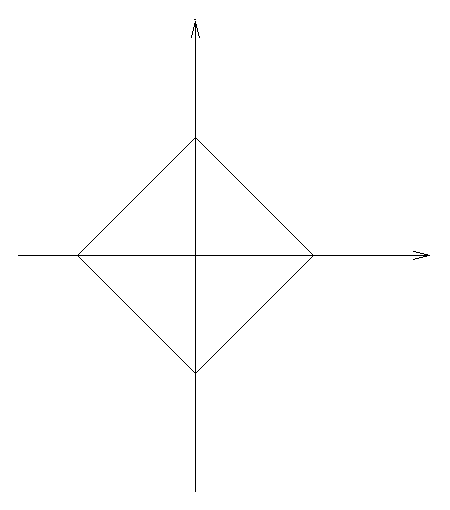
\includegraphics[width=5cm]{nrm1.eps} 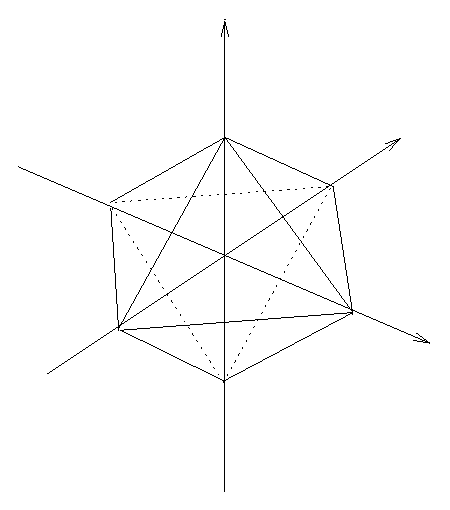
\includegraphics[width=5cm]{nrm13d.eps}}
\end{figure}

\subsubsection{Norme deux}

\begin{figure}[h]
	\centering{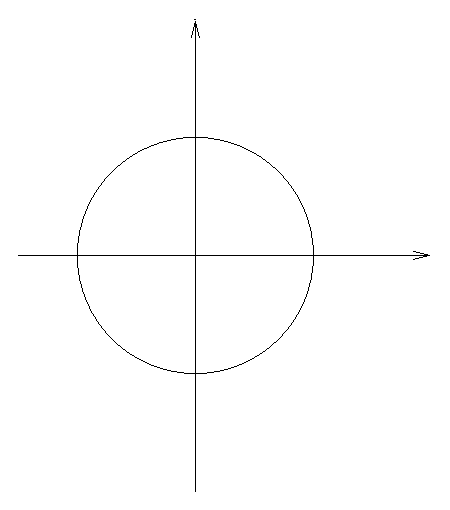
\includegraphics[width=5cm]{nrm2.eps} 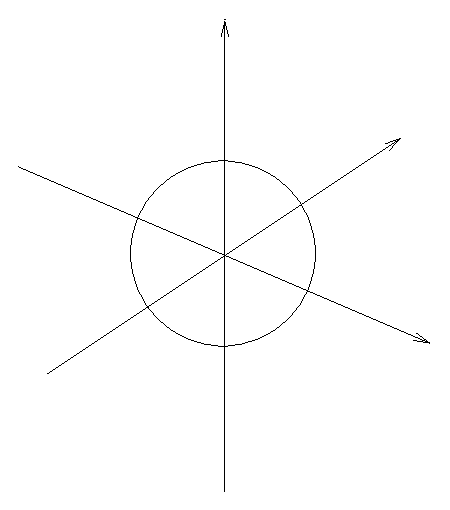
\includegraphics[width=5cm]{nrm23d.eps}}
\end{figure}

\newpage

\subsubsection{Norme infinie}

\begin{figure}[h]
	\centering{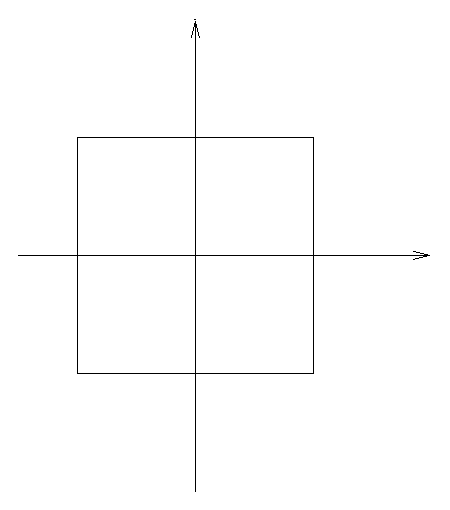
\includegraphics[width=5cm]{nrmi.eps} 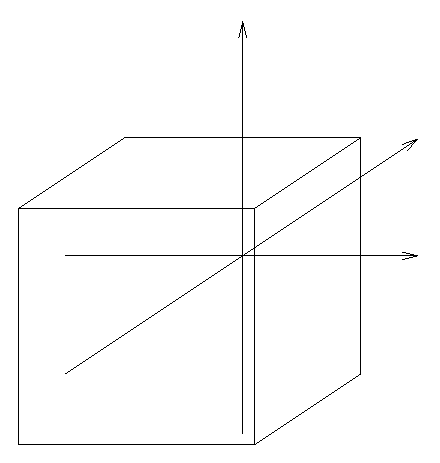
\includegraphics[width=5cm]{nrmi3d.eps}}
\end{figure}

\subsubsection{Normes un, deux et infinie imbriquées}

\begin{figure}[h]
	\centering{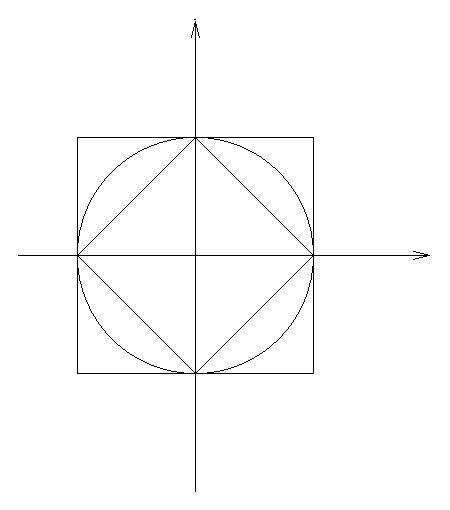
\includegraphics[width=5cm]{nrm12i.eps}}
\end{figure}


\subsection{Segment}

On note le segment allant de $x$ à $y$ dans $\R^N$ par $\left[ x,y \right]$

On définie $\left[ x,y \right]=\left\lbrace x + \lambda(y-x) \vert \lambda \in \left[ 0,1 \right] \right\rbrace = \left\lbrace (1-\lambda) x + \lambda y \vert \lambda \in \left[ 0,1 \right] \right\rbrace$

\subsection{Ensemble convexes}

Un ensemble est convexe s'il contient les segments joignants deux de ses points

i.e. $\forall x,y \in A, \forall \lambda \in \left[ 0,1 \right], (1-\lambda) x + \lambda y \in A$

\subsection{Boules convexes}

Toutes les boules sont convexes

\subsection{Convergence en terme de boules}

$x_n \ap a \ioi \forall \varepsilon > 0, \exists n_0, \forall n \geq n_0, x_n \in B_{\Vert . \Vert} \left[ a, \varepsilon \right]$

\subsection{Rudiments de topologie}

\subsubsection{Ensemble borné}

Un ensemble $A$ est borné ssi $\exists r > 0$ tq $A \subseteq B(0,r)$

\subsubsection{Complété}

On note le complété de $A$ l'ensemble de tous les éléments sauf ceux de $A$ par :

$\mathcal{C} A = A^\mathcal{C} = \R^N_A$

\subsubsection{Bord d'un ensemble}

On note $\Bd A$ le bord d'un ensemble

On a $\Bd A = \tset{x \in \R^N \vert (\exists (x_n) \subseteq A, x_n \ap x) \mbox{ et } (\exists (y_n) \subseteq \mathcal{C}A, y_n \ap x)}$

Autrement dit, un point appartient au bord d'un ensemble si on peut trouver à la fois une suite qui converge vers ce point tout en restant dans (appartenant à) cet ensemble et une suite qui converge vers ce point tout en restant hors (n'appartenant pas à) cet ensemble. 

Remarque : $\Bd A = \Adh A \but \Int A$

\subsubsection{Adhérence d'un ensemble}

On note $\Adh A$ l'adhérence d'un ensemble

On a $\Adh A = \tset{x \in \R^N \vert \exists (x_n) \subseteq A, x_n \ap x}$

Autrement dit, un point appartient à l'adhérence d'un ensemble si on peut trouver une suite dans cet ensemble qui converge vers ce point.

Remarque : $\Adh A = \Int A \cup \Bd A$

\subsubsection{Intérieur d'un ensemble}

On note $\Int A$ l'intérieur d'un ensemble

On a $\Int A = \mathcal{C} \tset{x \in \R^N \vert \exists(x_n) \subset \mathcal{C}A, x_n \ap x} = \tset{x \vert \exists r, B_{\Vert . \Vert} \left[ x,r \right] \subseteq A}$

Remarque : $\Int A = \Adh A \but \Bd A$

%% TODO: rajouter la convergence de suites de \C et \R^2

\subsubsection{Ensemble fermé}

On a $A$ fermé ssi $\Adh A = A$

ssi $\forall (x_n) \subseteq A, \forall x \in \R^N, x_n \ap x \so x \in A$

\subsubsection{Ensemble ouvert}

On a $A$ ouvert ssi $\Int A = A$

ssi $\forall x \in A, \exists r > 0$ tq $B(x,r) \subseteq A$

\subsubsection{Ensemble compact}

On a $A$ compact ssi $A$ est fermé et borné

Rmq: Tous les sensembles finis sont compacts

\section{Limite de fonctions et continuité}

\subsection{Limite en un point d'une fonction}

Soit $f: \R^N \ap \R^M$ et $a \in \Adh \Dom f$

$\clim{x\ap a} f(x) = b$ ssi $\forall (x_n) \subseteq \Dom f, x_n \ap a \so f(x_n) \ap b$

\subsubsection{Définition équivalente en termes de $\varepsilon , n_0$}

$\clim{x\ap a} f(x) = b$ ssi $\forall (x_n) \subseteq \Dom f, x_n \ap a \so \forall \varepsilon > 0, \exists n_0, \forall n \geq n_0, \Vert f(x_n) - b \Vert \leq \varepsilon$

\subsubsection{Définition équivalente en termes de $\varepsilon, \delta$}

$\clim{x\ap a} f(x) = b$ ssi $\forall \varepsilon > 0, \exists \delta >0, \forall x \in \Dom f, {\Vert x - a \Vert}_{\R^N} \leq \delta \so {\Vert f(x) -b \Vert}_{\R^M} \leq \varepsilon$

\subsubsection{Définition équivalente en termes de boules}

$\clim{x\ap a} f(x) = b$ ssi $\forall \varepsilon >0, \exists \delta>0,\forall x \in \Dom f, x \in B[a,\delta] \so f(x) \in B[b,\varepsilon]$

%%On note la limite en $a$ de $f(x)$ par $\lim\limits_{x \ap a} f(x)$

%%Cette limite vaut $b$ tel que si une suite $x_n \ap a \so f(x_n) \ap b$

\subsection{Procédés pour nier l'existence de la limite}

\begin{itemize}
	\item{Soit construire une suite $x_n \ap a$ tq $f(x_n)$ diverge}
	\item{Soit construire deux suites qui convergent vers $a$ tq les suites convergent par $f$ vers des valeurs $\neq$}
\end{itemize}

\subsection{Méthode pour trouver la limite}

\begin{itemize}
	\item[1]{En prenant un chemin particulier qui converge vers le point on peut voir la valeur de la limite (si elle existe)}
	\item[2]{Si la limite existe on sait qu'elle vaut la valeur trouvé en $1$}
        \item[3]{On prouve que la limite vaut bien cette valeur}	
\end{itemize}

\newpage

\subsubsection{Exemple}

$\clim{(x,y) \ap (0,0)} \frac{x^7 y^5}{x^4+y^4}$ ?

On veut trouver un chemin $(x_n,y_n) \ap (0,0)$

Prenons $x_n = \frac{1}{n}$

Prenons $y_n = \frac{1}{n}$

On a bien $x_n \ap 0$ et $y_n \ap 0$ donc $(x_n,y_n) \ap (0,0)$

On a alors $\clim{n \ap \infty} \frac{ (\frac{1}{n})^{12} }{2 (\frac{1}{n})^4 } = \clim{n \ap \infty} \frac{1}{2 n^8} = 0$

Donc si la limite existe, elle vaut $0$

On va montrer que la limite vaut bien $0$

Soit $(x_n,y_n) \ap (0,0)$

A-t-on $\forall \varepsilon > 0, \exists n_0, \forall n \geq n_0, \abs{ \frac{{x_n}^7 {y_n}^5}{{x_n}^4 + {y_n}^4}} \leq \varepsilon$

Soit $\varepsilon > 0$

Comme $y_n \ap 0$ on sait par hypothèse $\exists n_1, \forall n \geq n_1, \vert y_n \vert \leq 1$

Donc $\forall n \geq n_1 , \abs{ \frac{ {x_n}^7 {y_n}^5  }{ {x_n}^4 + {y_n}^4 } } \leq \abs{ \frac{x_n^7}{x_n^4 + y_n^4}} \leq \abs{ \frac{x_n^7}{x_n^4}} = \abs{x_n}^3$

Comme $x_n \ap 0$ on sait par hypothèse $\exists n_2, \forall n \geq n_2, \vert x_n \vert \leq \sqrt[3]{\varepsilon}$ càd ${\vert x_n \vert}^3 \leq \varepsilon$

Pour $n_0 = \max(n_1,n_2)$ on a $\forall n \geq n_0, \abs{ \frac{x_n^7 y_n^5}{x_n^4 + y_n^4 } } \leq {\vert x_n \vert}^3 \leq \varepsilon$ 
\subsubsection{Limite à droite}

On note la limite à droite $\lim\limits_{x \conv{\geq} a} f(x)$ (avec $x \geq a$ ou $\forall n, x_n \geq a$)

\subsubsection{Limite à gauche}

On note la limite à gauche $\lim\limits_{x \conv{\leq} a} f(x)$ (avec $x \leq a$ ou $\forall n, x_n \leq a$)

\subsubsection{Limite par valeurs différentes}

On note la limite par valeurs différentes $\lim\limits_{x \conv{\neq} a} f(x)$ 

(avec $x \neq a$ ou $\forall n, x_n \neq a$)

\subsection{Continuité en $a$}

Soit $f : \R^N \ap \R^M$ et $a \in \Dom f$

On dit que $f$ est continue en $a$ ssi :

$\forall (x_n) \subseteq \Dom f, x_n \ap a \so f(x_n) \ap f(a)$

%%Soit $a \in \Dom f$

%%Soit $b \in \R^M$

%%On dit que $f$ est continue en $a$ ssi 

%%$f(x) \ap b$ lorsque $x \ap a, x \in A$

%%$\Updownarrow$

%%$\forall (x_n), x_n \ap a \so f(x_n) \ap b = \lim\limits_{x \ap a} f(x)$

%%Ce qui est faux si on peut trouver une suite $(x_n)$ tq $x_n \ap a$ et $f(x_n)$ ne converge pas vers $b$

%%Remarque : $b$ est unique

%%Remarque : on dit $a \in \R^N \cap \Adh \Dom f \cap A$ afin d'être à même bord pour qu'on puisse avoir une suite $\subseteq \Dom f$ qui tend vers $a$

%\subsubsection{Définition équivalente}

%On a que $f$ est continue en $a \in \Dom f$ ssi $\clim{x \in \Dom f \ap a} f(x) = f(a)$

\subsection{Opération sur les fonctions}

Soit $f,g : \R^N \ap \R^M : x \mapsto f(x),g(x)$ deux fonctions

On définie 

\begin{itemize}
	\item{$f+g : \R^N \ap \R^M : x \mapsto f(x) + g(x) , \Dom (f+g) = \Dom f \cap \Dom g$}
	\item{$f . g : \R^N \ap \R^M : x \mapsto f(x).g(x), \Dom(f.g) = \Dom f \cap \Dom g$}
        \item{$f \rd g : \R^N \ap \R^M : x \mapsto f(g(x)), \Dom(f \rd g) = \Dom f \cap \Dom g$}	
\end{itemize}

\subsection{Opération sur les limites de fonctions}

Soit $f(x),g(x) : \R^N \ap \R^M : x \mapsto f(x),g(x)$ deux fonctions

Soit $a \in \Adh(\Dom f \cap \Dom g)$

Soit $\lim\limits_{x \ap a} f(x) = b$ 

Soit $\lim\limits_{x \ap a} g(x) = c$

Alors 

\begin{itemize}
	\item{$\lim\limits_{x \ap a} (f + g)(x) = b + c$}
	\item{$\lim\limits_{x \ap a} (f.g)(x) = b.c$}
	\item{Si $b \neq 0$ alors $\lim\limits_{x \ap a} \frac{1}{f(x)} = \frac{1}{b}$}
\end{itemize}


\subsection{Convergence dominée pour les fonctions}

Soit $f : \R^N \ap \R^M$

Soit $a \in \Adh \Dom f$

Soit $b \in \R^M$

Si il existe $g : \R^N \ap \R^M$ tel que $\Dom f \subseteq \Dom g$ et

$\exists r > 0, \forall x \in B[a,r] \cap \Dom f, \Vert f(x) - b \Vert \leq g(x)$

Tel que $\lim\limits_{x \ap a} g(x) = 0$

Alors $\lim\limits_{x \ap a} f(x) = b$

\subsubsection{Définition équivalente}

Soient $f,g : \R^N \ap \R^M$

Soit $a \in \R$

Si $\forall x \in \R^N, \Vert f(x) \Vert \leq \Vert g(x) \Vert$ et $\clim{x \ap a} g(x) = 0$

Alors $\clim{x \ap a} f(x) = 0$

%Non-sense :
%\subsection{Sandwich pour les fonctions}

%Soient $f,g,h : \R^N \ap \R^M$ et $a \in \R$

%Si $\Vert f(x) \Vert \leq \Vert g(x) \Vert \leq \Vert h(x) \Vert$

%Et $\clim{x \ap a} f(x) = b$

%Et $\clim{x \ap a} h(x) = b$

%Alors $\clim{x \ap a} g(x) = b$

\subsection{Fonctions de base}

Soit $\Vert. \Vert$ une norme et $a \in \R^N$

$\lim\limits_{x \ap a} \Vert x \Vert = \Vert a \Vert$

\subsection{Remarque}

$\clim{x\ap a} f(x) = b \ioi \clim{x \ap a} \Vert f(x)-b \Vert = 0$

\subsection{Lemme}

Si $a \in \Dom f$ soit $\clim{x \ap a} f(x) = f(a)$ soit $\clim{x \ap a} f(x)$ n'existe pas

%%\subsection{Lemme}
 
%%Soit $(x_n)$ et $(y_n)$

%%Si $x_n \ap a$

%%Si $y_n \ap a$

%%Et si $f(x_n) \ap b$

%%Et si $f(y_n) \ap c$

%%Avec $b \neq c$

%%Alors $\clim{x \ap a} f(x)$ n'existe pas

\subsection{Lemme}

Si $A \subseteq B$

Si $\clim{x \in B \ap a} = b$ existe

Alors $\clim{x \in A \ap a}$ existe et vaut $b$

\subsection{Diagonale}

On note la diagonale $\Delta = \tset{(x,y) \vert x = y}$

%\subsection{Fonction continue en un point}

%Soit $f : \R^N \ap \R^M, a \in \Dom f$

%On dit que $f$ est continue en $a$ 

%ssi $\clim{x\ap a} f(x) = f(a)$

%ssi $f(x) \conv{x \ap a} f(a)$

%ssi $\clim{x \ap a} f(x) \exists$

%Cette limite vaut nécessairement $f(a)$ car $a \in \Dom f$ 

%Remarque: $a \not \in \Dom f$ alors on ne parle pas de continuité en $a$

\subsection{Opération sur les fonctions continues}

\subsubsection{Somme}

Soit $f,g : \R^N \ap \R^M$ et $a \in \Dom f \cap \Dom g$

Si $f$ et $g$ sont continues en $a$ alors $f+g$ est continue en $a$

\subsubsection{Produit}

Soit $f : \R^N \ap \R^M$ , $g : \R^N \ap \R$ et $a \in \Dom f \cap \Dom g$

Si $f$ et $g$ sont continues en $a$ alors $f.g : \R^N \ap \R^M$ est continue en $a$

\subsubsection{Quotient}

Soit $f : \R^N \ap \R^M$ , $g : \R^N \ap \R$ et $a \in \Dom f \cap \Dom g$

Si $f$ et $g$ sont continues en $a$ et $g(a) \neq 0$ alors $f/g : \R^N \ap \R^M$ est continue en $a$

\subsubsection{Composition}

Soit $f,g$ deux fonctions tq $\R^N \conv{f} \R^M \conv{g} \R^P$

Avec $a \in \Dom f, f(a) \in \Dom g$

Alors $g \circ f : \R^N \ap \R^P : x \mapsto f(x) \mapsto g(f(x))$ est continue en $a$

\subsection{Propriété}

%% FIXME: Son nom ? Continuité dominée ?

Si $f : \R^N \ap \R^M$ , $g : \R^N \ap \R$ et $a \in \Dom f \cap \Dom g$ tq

$\exists \varphi > 0, \forall x \in B(0,\varphi), \Vert f(x) - f(a) \Vert \leq g(x)$

et $g(x) \conv{x \ap a} 0$, alors $f$ est continue en $a$

\subsection{Fonction continue sur un ensemble}

Une fonction $f: \R^N \ap \R^M$ est continue sur $A$ si quelque soit $a \in \Dom f \cap A$, $f$ est continue en $a$

\subsection{Fonction continue}

Une fonction $f: \R^N \ap \R^M$ est continue si quelque soit $a \in \Dom f$, $f$ est continue en $a$

Autrement dit $f$ est continue ssi $f$ est continue en tout points de son domaine

\subsubsection{Exemples de fonctions continues}

\begin{itemize}
	\item{$\Vert . \Vert : \R^N \ap \R$}
	\item{$\mathbb{I} : \R \ap \R : x \mapsto x$}
	\item{$p_i : \R^N \ap \R : (x_1, \dots, x_N) \mapsto x_i$}
	\item{Les application linéaires en dimension finie}
	\item{Les polynomes sont continues sur $\R$}
	\item{$f : \R \ap \R : x \mapsto \frac{1}{x}$ est continue}
	\item{$\sin x, \cos x, \tan x, \arctan x, \arcsin x, e^x, \dots $}
\end{itemize}

\subsubsection{Exemples de fonctions non continues}

\begin{itemize}
	\item{$f: \R \ap \R : x \mapsto \begin{cases} \frac{1}{x} & \mbox{si } x \neq 0 \\ 0 & \mbox{sinon} \end{cases}$}
	\item{$f: \R \ap \R : x \mapsto \begin{cases} 1 & \mbox{si } x > 0 \\ 0 & \mbox{sinon} \end{cases}$}
\end{itemize}

\subsection{Remarque}

Une fonction définie par parties dont les fonctions qui la définissent sont continues n'est pas forcément continue

%\subsection{Intervale}

%Soit $a, b \in \R$ on note l'ensemble des points entre $a$ et $b$ par 

%$[a, b] = 
%\begin{cases}
%	\tset{x \vert a \leq x \leq b} & \mbox{si } a \leq b \\
%	\tset{x \vert a \geq x \geq b} & \mbox{si } a \geq b
%\end{cases} = \tset{ta + (1 - t) b \vert t \in [0,1]}$ 

%\subsection{Théorème des valeurs intermédiaires}

%Si $f : [a, b] \ap \R$ est continue et définie sur $[a, b]$ alors $[f(a), f(b)] \subseteq f([a,b])$

%Càd $\forall l \in [ f(a), f(b) ] , l \in f([a,b])$

%Càd $\exists x \in [a,b], l = f(a)$

\subsection{Connexe par arc}

Un ensemble $A \subseteq \R^N$ est connexe par arc $\forall x,y \in A$ je peux aller de $x$ à $y$ par un chemin $\gamma$

Càd $\forall x,y \in A, \exists \gamma : [0,1] \ap A$ continue tq $\gamma(0) = x, \gamma(1) = y$

Remarque : L'idée de connexité c'est un ensemble en un seul morceau


\subsection{Théorème des valeurs intermédiaires}

Si $f : [a,b] \ap \R$ continue et $f(a).f(b) < 0$ alors $\exists \xi \in ]a,b[, f(\xi) = 0$

Si $f : [a,b] \ap \R$ continue et $f(a).f(b) \leq 0$ alors $\exists \xi \in [a,b], f(\xi) = 0$

\subsubsection{Remarque}

Il faut $\R$ pour ce théorème.

Prenons $f: \Q \ap \R : x \mapsto x^2 - 2$ par exemple on a $f(0) < 0, f(2) > 0$ mais $\forall \xi \in \Q, f(\xi) \neq 0$

\newpage

\subsubsection{Remarque}

Le théorème des valeurs intermédiaires nous dit qu'il existe \textit{au moins} une racine. Donc il peut en exister plus qu'une voir une infinitée.

Prenons par exemple $f:[0,1] \ap \R : x \mapsto \begin{cases} x \sin \frac{1}{x} & \mbox{si } x \neq 0\\ 0 & \mbox{sinon}\end{cases}$  

\begin{figure}[h]
	\centering{\epsfig{figure=xsinx.eps,width=10cm}}
\end{figure}

\subsection{Théorème des valeurs intermédiaires général}

Si $f : [a, b] \ap \R$ continue et $l \in [f(a),f(b)]$ alors $\exists \xi \in [a,b]$ tq $f(\xi) = l$


\subsection{Théorème des valeurs intermédiaires à $N$-dimensions}

Si $f : D \subseteq \R^N \ap \R$ continue et $a,b \in D$ tq $f(a) < 0 < f(b)$ et $D$ connexe (par arcs) alors :

$\exists \xi \in D$ tq $f(\xi) = 0$

\section{Différenciabilité}

\subsection{Quotient différentiel}

On appelle $\clim{x \ap a} \frac{f(x) - f(a)}{x -a}$ le quotient différentiel

\subsection{Fonction dérivable en un point}

Soit $f : \Dom f \subseteq \R \ap \R$ et $a \in \Adh ( \Dom f \but \tset{a} )$

On dit que $f$ est dérivable en $a$ ssi $\clim{x \conv{\neq} a} \frac{f(x) - f(a)}{x-a}$ existe

%Si cette limite existe on l'appelle la dérivée de $f$ en $a$ et on la note $f(a) , \partial f(a) , \frac{df}{dx}(a)$
Si cette limite existe on l'appelle la dérivée de $f$ en $a$ et on la note $f'(a), \partial_x f(a) , \frac{df}{dx}(a)$

\subsubsection{Remarque}

On prend $a \in \Adh(\Dom f \but \tset{a})$ pour éviter de prendre les points isolés qui appartiennent au domaines.

Autrement dit on prend les points appartenant au domaines avec son bord sauf les points isolés.

On peut aussi dire $a \in \Int (\Dom f)$

\subsubsection{Remarque}

$\partial f(a)$ est la pente de la tangente au graphe de $f$ passant par $(a,f(a))$

\subsubsection{Proposition}

Si $f$ est dérivable en $a$ alors $f$ est continue en $a$

\subsection{Tangente}

Soit $f : \R \ap \R$ dérivable en $a$

On note la tangente au point $a$ de $f$ par

$T \equiv y = f(a) + \partial f(a) (x - a)$

\begin{figure}[h]
	\centering{\epsfig{figure=tgt.eps,width=5cm}}
\end{figure}

\subsection{Petit $o$ de $x-a$ lorsque $x \ap a$}

On dit qu'une fonction $g$ est un petit $o$ de $(x-a)$ lorsque $x \ap a$ ssi :

$\begin{cases}
	\clim{x \ap a} \frac{g(x)}{x-a} = 0\\
	g(a) = 0 \mbox{ si } a \in \Dom f
\end{cases}$

Ce qu'on note $g(x) = o(x-a)$

\subsubsection{Remarque}

C'est un abus de notation car $o(x-a)$ représente une classe de fonctions.

Autrement dit quand on note $o(x-a)$ on sous entend une fonction qui est un $o$ de $x-a$ mais qui peut changer à chaque occurence.

On a donc en particulier $o(x-a) + o(x-a) = o(x-a)$ ce qu'on peut traduire par :

Si $g_1$ et $g_2$ sont $o$ de $x-a$ alors $g_1 + g_2$ l'est encore.

\subsubsection{Remarque}

Si $g = o(x-a)$ alors $g(x) \conv{x \ap a} 0$

\subsubsection{Fonction bornée au voisinage d'un point}

Soit $g : \R^N \ap \R$ et $a$ dans $\R^N$, on a que $g$ est bornée au voisinage de $a$ ssi :

$\exists C > 0, \forall x \in B(a,C), \abs{g(x)} \leq C$


\subsubsection{Opérations sur les $o(x-a)$}

Soit $g : \R \ap \R$ bornée au voisinage de $a$

\begin{itemize}
	\item{$o(x-a)+o(x-a)=o(x-a)$}
        \item{$o(x-a).o(x-a) = o(x-a)$}
        \item{$o(x-a).g(x) = o(x-a)$}
\end{itemize}

\subsection{Définition équivalente de la dérivabilité}

On a que $f$ est dérivable en $a \ioi \exists a', b' \in \R$ tq $f(x) - (a'x + b') = o(x-a)$

Autrement dit on a que $f$ est dérivable en $a$ ssi la tangente au point $(a,f(a))$ existe

Si une des deux propositions est vérifiée on a alors :

$a' = \partial f(a)$ et $b' = f(a)-a.\partial f(a)$

\subsubsection{Propositions}

Soit $f,g$ deux fonctions dérivables en $a$

\begin{itemize}
	\item{$f+g$ est dérivable en $a$}
	\item{$f.g$ est dérivable en $a$}
	\item{Si $g(a) \neq 0$, alors $f/g$ est dérivable en $a$}
\end{itemize}

\subsubsection{Opérations sur les dérivées}

Soit $f,g$ deux fonctions dérivables en $a$

\begin{itemize}
	\item{$\partial(f+g)(a) = \partial f(a) + \partial g(a)$}
	\item{$\partial(f.g)(a) = g(a).\partial f(a) + f(a).\partial g(a)$}
	\item{$\partial(f/g)(a) = \frac{g(a).\partial f(a) - f(a).\partial g(a)}{g(a)}$}
	\item{$\partial(f \circ g)(a) = \partial f(y) . \partial g(a) \vert y = f(a)$}
\end{itemize}

\subsection{Petit $o$ de $k$ lorsque $x \ap a$}

On a que $h$ est un petit $o(k)$ lorsque $x \ap a$ ssi 

$\begin{cases}
	\frac{h(x)}{k(x)} \conv{x \ap a} 0\\
	k(a) = 0 \so h(a)=0
\end{cases}$

\subsection{Petit $o$ de $(x-a)^k$ lorsque $x \ap a$}

On a $f: \R \ap \R$ est $o\left( \left( x-a \right)^k \right)$ quand $x \ap a$ ssi 

$\begin{cases}
	\clim{x \ap 0} \frac{f(x)}{h(x)} = 0\\
	f(a) = 0
\end{cases}$

\subsubsection{Interprétation}

Autour de $a$, la fonction file vers $0$ plus vite que $\left( x -a  \right)^k$ ou $-\left( x-a \right)^k$ 

\subsubsection{Remarque}

$h$ est $o(1)$ qd $x \ap a \ioi h(x) \clim{x \ap a} h(x) = 0$ et $h(a) = 0$

Donc on a aussi $h(x) = o\left( \left( x-a \right)^k \right)$ ssi $h(x) = \left( \left( x-a \right)^k \right).o(1)$

\subsubsection{Proposition}

$h$ est $o(k)$ qd $x \ap a \ioi h = o(1).k$

Autrement dit :

$h$ est $o(k) \ioi \exists l$ un $o(1)$ tq $h=l.k$

\subsection{Fonction inverse}

La fonction inverse\footnote{A ne pas confondre avec $1/f$} de $f : I \subseteq \R \ap J \subseteq \R$ si elle existe est une fonction $g : J \ap I$ tq $f \circ g = \Id_J$ et $g \circ f = \Id_I$ càd $\forall j \in J f(g(j)) = j$ et $\forall i \in I g(f(i)) = i$

Si l'inverse existe, il est unique et se note $f^{-1}$

\subsection{Proposition}

Si $f$ est inversible et $f,f^{-1}$ sont dérivables alors $\partial f(x) \neq 0$ pour tout $x \in I$ et $\partial_y f^{-1} f(y) = \frac{1}{(\partial_x f)(f^{-1}(y)}$

En fait si $f$ est dérivable et inversible sur $I$ alors son inverse est dérivable sur $J$

\subsection{Théorème des bornes atteintes}

Si $\Omega \subseteq \R^N$ compact et $f : \Omega \ap \R$ une fonction continue alors :

$\exists x_{\min}, x_{\max} \in \Omega : \forall x \in \Omega ; f(x_{\min}) \leq f(x) \leq f(x_{\max})$

Autrement dit sur un compact, une fonction continue atteint ses bornes

\subsubsection{Minimum local}

Si $f: [ a, b ] \subseteq \R$ et $x^\star \in [a,b]$

On dit que $x^\star$ est un minimum local si :

$\exists \varphi > 0, \forall x \in B(x^\star,\varphi), f(x^\star) \leq f(x)$

\subsubsection{Maximum local}

Si $f: [ a, b ] \subseteq \R$ et $x^\star \in [a,b]$

On dit que $x^\star$ est un maximum local si :

$\exists \varphi > 0, \forall x \in B(x^\star,\varphi), f(x^\star) \geq f(x)$

\subsubsection{Minimum global}

Si $f: [ a, b ] \subseteq \R$ et $x^\star \in [a,b]$

On dit que $x^\star$ est un minimum global si :

$\forall x \in [a,b], f(x^\star) \leq f(x)$

\subsubsection{Maximum local}

Si $f: [ a, b ] \subseteq \R$ et $x^\star \in [a,b]$

On dit que $x^\star$ est un maximum local si :

$\forall x \in [a,b], f(x^\star) \geq f(x)$

\subsection{Proposition}

Si $f: ]a,b[ \ap \R$ est dérivable et $\xi \in ]a,b[$ est un minimum ou un maximum local alors $\partial f(\xi) = 0$

\subsection{Théorème de Rolle}

Si $f : [a,b] \ap \R$ est continue sur $[a,b]$ et dérivable sur $]a,b[$ tq $f(a) = f(b)$ alors $\exists \xi \in ]a,b[, \partial f(\xi) = 0$

\subsection{Théorème de la moyenne}

Si $f: [a,b] \ap \R$ continue sur $[a,b]$ et dérivable sur $]a,b[$ alors $\exists \xi \in ]a,b[$ tq $f(b) - f(a) = \partial f(\xi) (b-a)$

\subsubsection{Corrolaire du théorème de la moyenne}

\begin{itemize}
	\item{$f$ croissante sur $[a,b] \ioi \forall x \in ]a,b[, \partial f(x) \geq 0$}
         \item{$f$ décroissante sur $[a,b] \ioi \forall x \in ]a,b[, \partial f(x) \leq 0$}
         \item{$\partial f(x) > 0 \so f$ strictement croissante}
         \item{$\partial f(x) < 0 \so f$ strictement décroissante}
\end{itemize}

\subsection{Classe $\mathcal{C}^k$}

On a que $f$ est de classe $\mathcal{C}^k, k \geq 2$ ssi $f$ est $k$ fois dérivable sur $I$ et $I \so \R: x \ap \partial^k f(x)$ est continue

On note $f \in \mathcal{C}^k (I;\R)$

On note $f \in \mathcal{C}^0 (I;\R) = \mathcal{C} (I ; \R)$ si $f$ est continue sur $I$ et $\partial^0 f = f$

On note $\cclass{\infty}{I}{\R} = \bigcap\limits_{k\in \N} \cclass{k}{I}{\R} = \tset{f : I \ap \R \vert \forall k \in \N, \partial^k f \mbox{ existe et est continue} }$

On a $\cclass{\infty}{I}{\R} \subseteq \dots \cclass{k}{I}{\R} \subseteq \dots \subseteq \cclass{2}{I}{\R} \subseteq \cclass{1}{I}{\R} \subseteq \cclass{0}{I}{\R}$

\subsubsection{Remarque}

On a $\cclass{k}{I}{\R}$ est un sous espace vectoriel de $\R^I = \tset{f \vert f:I \ap \R}$


\subsection{Polynômes}

On note $\Poly^k = \tset{p \vert p \mbox{ est un polynôme de degré } \leq k}$

Ce qu'on peut traduire par :

$\Poly^k = \tset{p(x) \vert p(x) = \sum_{i=0}^{k} p_i \left( x-a \right)^i}$

On a $\Poly^k$ est un sous-espace vectoriel de dimension $k+1$

\subsection{Développement de Taylor}

Le développement de Taylor de $f$ en $a$ d'ordre $k \geq 0$ est le polynôme $p \in \Poly^k$ tq:

$f(x) - p(x) = o\left( \left( x-a \right)^k \right), x \ap a$ où $g = o\left( \left( x-a \right)^k \right)$ ssi $\frac{g(x)}{\left( x-a \right)^k} \conv{x \ap a} 0$

On a que si le développement de Taylor existe alors il est unique

\subsubsection{Opérations avec les DT}

Soit $p$ le DT d'ordre $m$ de $f$ en $a$ et $q$ le DT d'ordre $m$ de $g$ en $a$

Soit $q'$ le DT d'ordre $m$ de $g$ en $f(a)$

Alors on a :

\begin{itemize}
	\item{$p+q$ est le DT d'ordre $m$ de $f+g$ en $a$}
	\item{$p.q$ est le DT d'ordre $m$ de $f.g$ en $a$}
	\item{$q' \rd p$ est le DT d'ordre $m$ de $g \rd f$ en $a$}
\end{itemize}
\paragraph{Remarque :} Pour obtenir le DT d'ordre $m$ de $p.q$ et $q' \rd p$, il faut tronquer les termes de degrés plus haut que $m$ dans le polynôme obtenu.

\subsubsection{Formule du reste}

Soit $n \in \N$

Soit $I$ intervalle ouvert de $\R$

Soit $f : I \ap \R$ avec $f \in \cclass{n+1}{I}{\R}$

Soit $a \in I$

Alors $\forall x \in I, \exists \xi \in \left[ a,x \right]$ tq:

$$f(x) = \underbrace{\sum_{i=0}^n \frac{\partial^i f(a)}{i!} (x-a)^i}_{\mbox{DT}} + \underbrace{\frac{\partial^{n+1} f(\xi)}{\left( n+1 \right)!} \left( x-a \right)^{n+1}}_{o\left( \left( x-a \right)^n \right) \newline \mbox{ càd le reste}}$$

Remarque :

\begin{itemize}
	\item{C'est une généralisation du théorème de la moyenne}
	\item{$\partial^0 f = f$ par définition}
	\item{Ici $0^0 = 1$ (normalement cas d'intermination)}
	\item{Pour $n = 0$ on lit $\forall x \in I, \exists \xi \in \left[ a,x \right]$ tq $f(x) = f(a) + \partial f(\xi)(x-a)$}	
\end{itemize}

\subsubsection{Théorème}

Soit $f : \R \ap \R$ et $a \in \Dom f$ avec $n \in \N$.

Si il existe un voisinage $V$ de $a$ tq $f \in \cclass{n}{V}{\R}$ alors le DT d'ordre $n$ de $f$ en $a$ vaut 

$$p(x) = \sum_{i=0}^n \frac{\partial^i f(a)}{i!} \left( x-a \right)^i$$

\subsubsection{Exemples}

\begin{itemize}
	\item{Le DT d'ordre $n$ en $0$ de $e^x$ est $\displaystyle p(x) = \sum_{i=0}^n \frac{x^i}{i!}$}
	\item{Le DT d'ordre $n$ en $0$ de $\sin x$ est $\displaystyle p(x) = \sum_{i=0}^{\frac{n-1}{2}} \frac{(-1)^i x^{2 i + 1}}{(2 i + 1)!}$}
	\item{Le DT d'ordre $n$ en $0$ de $\cos x$ est $\displaystyle p(x) = \sum_{i=0}^{\frac{n}{2}} \frac{(-1)^i x^{2 i}}{(2i)!}$}
\end{itemize}

\section{Série}

Une série est une écriture symbolique du type $\sum_{n=n_0}^{+\infty} x_n$ où $(x_n)_{n \geq n_0}$ est une suite de $\R^N$ avec la notation suivante :

$$\sum_{n=n_0}^{+\infty} x_n = \clim{m \ap + \infty} \sum_{n=n_0}^m x_n$$

\subsubsection{Convergence}

Une série $\sum_{n=n_0}^{+\infty} x_n$ converge ssi la suite des sommes partielles $\left( \sum_{n = n_0}^m x_n \right)_{m \geq n_0}$ converge

\subsubsection{Proposition}

$$\sum_{n=n_0}^{+\infty} x_n \mbox{ converge } \so x_n \ap 0$$

$$x_n \nconv{~} 0 \so \sum_{n=n_0}^{+\infty} x_n \mbox{ diverge}$$

\subsubsection{Convergence absolue}

Une série converge \textit{absolument} ssi $\series \Vert x_n \Vert$ converge

\subsubsection{Proposition}

$$\series x_n \mbox{ converge absolument } \so \series x_n \mbox{ converge}$$

\subsubsection{Critère de convergence dominée}

Soient $\left( x_n \right)_{n\geq n_0} \subseteq \R^N$ et $\left( y_n \right)_{n \geq n_0} \subseteq \R$ tq $\Vert x_n \Vert \leq y_n$

$$\series y_n \mbox{ converge } \so \series x_n \mbox{ converge absolument }$$

\subsubsection{Critère d'équivalence}

Si $a_n \equiv b_n$ alors $\displaystyle \series a_n$ converge ssi $\displaystyle \series b_n$ converge

\subsubsection{Critère de d'Alembert}

\begin{itemize}
	\item{Si $\displaystyle \clim{n \ap +\infty} \frac{\abs{a_{n+1}}}{\abs{a_n}} < 1$ alors $\displaystyle \series a_n$ converge}
	\item{Si $\displaystyle \clim{n \ap +\infty} \frac{\abs{a_{n+1}}}{\abs{a_n}} > 1$ alors $\displaystyle \series a_n$ diverge}
	\item{Si $\displaystyle \clim{n \ap +\infty} \frac{\abs{a_{n+1}}}{\abs{a_n}} = 1$ alors on ne sait pas}
\end{itemize}

\subsubsection{Critère de Cauchy}

\begin{itemize}
	\item{Si $\displaystyle \clim{n \ap +\infty} \sqrt[n]{\abs{a_n}} < 1$ alors $\displaystyle \series a_n$ converge}
	\item{Si $\displaystyle \clim{n \ap +\infty} \sqrt[n]{\abs{a_n}} > 1$ alors $\displaystyle \series a_n$ diverge}
	\item{Si $\displaystyle \clim{n \ap +\infty} \sqrt[n]{\abs{a_n}} = 1$ alors on ne sait pas}
\end{itemize}

\subsubsection{Exemples de séries}

\begin{itemize}
	\item{$\displaystyle \Series{0} a^n$ converge ssi $\abs{a} < 1$}
	\item{$\displaystyle \Series{1} \frac{1}{n^\alpha}$ converge ssi $\alpha > 1$}
\end{itemize}





\section{Equation différentielles}

\subsection{Equation différentielle ordinaire}

Une EDO ou ODE (Ordinal Differential Equation) est une équation différentielle avec des dérivées en une seule variable du type :

$$f\left(t, \partial^n_t x,\partial^{n-1}_t x,\dots,\partial_t x,x \right) = 0$$

Avec $f : \R \times (\R^N)^{n+1} \ap \R^N$ et $x : \R \ap \R^N$

Par exemple l'équation : 

$$\partial_t x - x = 0$$

Est l'équation $f(t, \partial_t x,x) = 0$ avec $f(t,a,b)=a-b \in \R$

Où $n = 1$ et $N = 1$

\subsection{Solution d'une EDO}

Soit $f\left(t, \partial^n_t x,\partial^{n-1}_t x,\dots,\partial_t x,x \right) = 0$ avec $f : \R \times (\R^N)^{n+1} \ap \R^N$ et $x : \R \ap \R^N$ une EDO.

Une solution de cette équation est une fonction $X:]a,b[ \subseteq \R \ap \R^N$ tq :

\begin{itemize}
	\item{$\forall t \in ]a,b[, \partial_t^i x(t)$ existent pour $i=1,\dots,n$}
	\item{$\forall t \in ]a,b[, f\left( t,\partial_t^n x, \partial_t^{n-1} x, \dots,x\right) = 0$} 
\end{itemize}


\subsection{Remarque}

Soit $a,b \in \R$

On a $e^{a+bi} = e^a (\cos b + i \sin b)$


\subsection{EDO linéaires à coeff. constants}

Une EDO est linéaire si elle peut s'écrire sous la forme :

$$\sum_{i=0}^n a_i \partial^i_t x(t) = f(t)$$

Avec $\forall i \in \left\{0,\dots,n \right\} a_i \in \C$

On a alors une application linéaire :

$$Lx : \sum_{i=0}^n a_i \partial^i_t x(t) \mapsto f(t)$$

Comme $L$ est linéaire si on a une solution particulière $x_p$ de $Lx = f$

Alors l'ensemble des solutions est $x_p + \ker L$

\subsubsection{EDO linéaire homogène }

On appelle \eqdo linéaire homogène l'équation :

$$Lx = 0$$

L'ensemble des solutions de cette équation vaut $\ker L$

Les solutions de cette équation sont de la forme :

$$\sum_{i=1}^k p_i(t) e^{\lambda_i t}$$

Avec les $\lambda_1, \dots, \lambda_k$ les solutions complexes du poly. caractéristique $P(z)$ de $Lx$:

$$P(z) = \sum_{i=0}^n a_i z^i = 0$$

Avec les $p_1,\dots,p_k$ des polynômes à coefficients dans $\C$ où $\mbox{deg } p_i < m_a(\lambda_i)$ 

Où $m_a(\lambda_i)$ est la multiplicité algèbrique de $\lambda_i$ comme racine de $P(z)$ 

%% RESTE AVEC P(z) et coeff de p_i

\subsubsection{Proposition}

Si $Lx = \sum_{i=0}^n a_i \partial^i x$ avec $a_i \in \R$ pour $i = 0,\dots,n$ alors :

$$\tset{x:\R \ap \R \vert L(x) = 0}$$

$$ = \tset{\mbox{Re } x \vert x : \R \ap \C \mbox{ tq } L(x) = 0}$$

$$ = \mbox{Re }(\alpha e^{\sqrt{a} i t} + \beta e^{- \sqrt{a} i t})$$

\subsubsection{Forme particulière}

Soit une \eqdo de la forme :

$$Lx = \sum_{j=1}^k q_j(t) e^{\mu_j t}$$

Avec $q_j(t)$ un polynôme à coefficients dans $\C$ et $\mu_j \in \C$

On a que si $x_j$ est solution de $Lx_j = q_j e^{\mu_j t}$

Alors $\sum_{j=1}^k x_j$ est solution de $Lx = \sum_{j=1}^k q_j(t) e^{\mu_j t}$

\subsubsection{Théorème}

Soit une \eqdo de la forme :

$$Lx = q e^{\mu t}$$

Une solution particulière de cette équation est :

$$r(t) t^\alpha e^{\mu t}$$

Avec $r$ est un polynôme tq $\deg r \leq \deg q$

Avec $\alpha$ la multiplicité de $\mu$ comme racine de $p$

Pour trouver $r$ on injecte la solution particulière dans l'équation et on résoud le système linéaire en les coefficients de $r$

\subsection{EDO à variables séparées}

Soit $h,g : \R \ap \R$

Une EDO à variables séparées est de la forme :

$$\partial_t u(t) = h(t) g(u(t))$$

avec $u : \R \ap \R$

%% TODO Méthode de variation des constantes

\subsubsection{Solution d'une \eqdo à variable séparées}

Soit une \eqdo à variable séparées de la forme :

$$\partial_t u = h(t) g(u)$$

On a :

$$\int_{t_0}^t \frac{\partial_t u}{g(u)} dt = \int_{t_0}^t h(t) dt$$

Rmq : on suppose $g(u) \neq 0$

Posons $\xi = u(t)$ et $d \xi = \partial_t u(t) dt$ (on peut car $u$ est inversible et $u \in \mathcal{C}^1$)

On a :

$$\int_{u(t_0)}^{u(t)} \frac{1}{g(\xi) d \xi} = \int_{t_0}^t h(t) dt$$

Notons $G$ la primitive de $1/g$ et $H$ la primitive de $h$

Alors on a :

$$G \vert_{u(t_0)}^{u(t)} = G(u(t)) - G(u(t_0)) = H(t)$$

Comme $G$ est strictement monotone on a $G$ inversible

Donc :

$$u(t) = G^{-1}(G(u(t_0)) + H(t))$$


%%Càd :

%%$$\ln u(t) - \ln u(t_0) = \int_{t_0}^t h(t) dt$$

%%Mais comme $\ln e^t = t$ on a :

%%$$u(t) = e^{\ln u(t_0) + \int_{t_0}^t h(t) dt}$$

\subsubsection{Primitive}

On a $F$ est primitive de $f$ ssi $\partial F = f$

De plus si $F_1$ et $F_2$ sont deux primitives de $f$ alors :

$$\exists c \in \R, \forall t, F_1 (t) = c + F_2(t)$$

Car on a $\partial(F_1 - F_2) = \partial F_1 - \partial F_2 = f - f = 0 \so F_1 - F_2 = c$

\subsubsection{Théorème fondamental de l'analyse}

Si $F$ est primitive de $f$ 

Alors $\int_a^b f(t) dt= F(b) - F(a)$

Càd $\partial_t \int_a^t f(t) dt = f(t)$

\subsubsection{Intégration par substitution}

Soit une fonction $u(t)$ (même non inversible) alors on a :

$$\int_a^b K(u(t)) \partial_t u(t) dt = \int_{u(a)}^{u(b)} K(s) ds$$

\subsection{Théorème d'existence et d'unicité}

Soit une équation du type $\partial_t^k u = f(t, \partial_t^{k-1} u, \dots,\partial_t u, u)$

Avec $f$ continue et $f(t,u_{k-1},\dots,u_1,u_0)$ est dérivable par rapport à $t,u_{k-1},\dots,u_1,u_0$

Et ces dérivées sont continues

Alors $\forall t_0$ et $v_{k-1},\dots,v_1,v_0$

Il existe une et une seule solution de cette équation

$$u:]t_0 - \varepsilon,t_0 + \varepsilon[ \ap \R$$

Telle que 

$$\partial^{k-1}_t u(t_0) = v_{k-1}, \dots \partial_t u(t_0) = v_1, u(t_0) = v_0$$

\end{document}
